\documentclass{standalone}

\usepackage{tikz}
\usepackage{tikz-qtree}
\usepackage{../../../texmf/tex/latex/mathoperators/mathoperators}

\begin{document}
	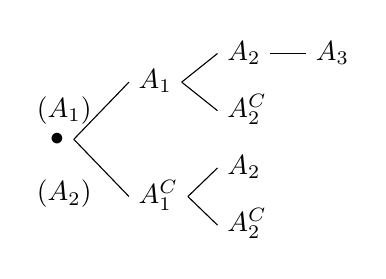
\begin{tikzpicture}
	\tikzset{grow'=right,level distance=32pt}
	\tikzset{execute at begin node=\strut}
	\tikzset{every tree node/.style={anchor=base west}} %TODO add better node placing and the rest of the nodes!
	\Tree [.$\bullet$ 
		\edge node[midway,left]{$\probp(A_1)$}; 
		[.$A_1$ [.$A_2$ $A_3$ ] [.$A_2^C$ ] ]
	\edge node[auto=right]{$\probp(A_2)$};
		[.$A_1^C$ [.$A_2$ ]
			[.$A_2^C$
				 ] ] ]
	\end{tikzpicture}
\end{document}